\question{Механизм создания инверсной населенности уровней в трехуровневой системе. Способы накачки}

\begin{figure}[h]
\begin{center}
    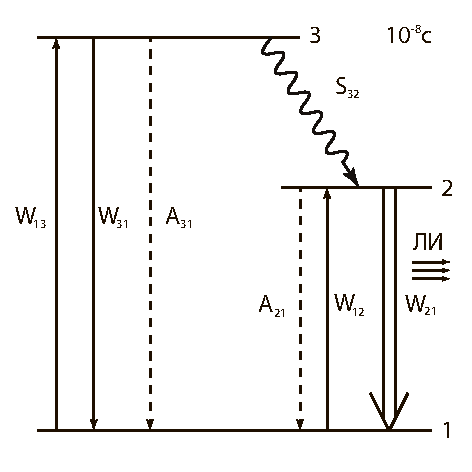
\includegraphics[width=.47\textwidth]{10_1}
\end{center}
\end{figure}

Рассмотрим стационарный режим в трёхуровневой системе:
\begin{align*}
    & \der{N_3}{t} = W_{13}N_1 - (W_{31} + A_{31} + S_{32}) N_3 = 0,\\
    & \der{N_2}{t} = S_{32}N_3 + W_{12}N_1 - (A_{21} + W_{21}) N_2 = 0,\\
    & N_1 + N_2 + N_3 = \const = N_0.
\end{align*}
Свяжем \( N_1 \) и \( N_2 \). Из первого уравнения выразим \( N_3 \)
\[
    N_3 = \frac{W_{13}N_1}{W_{31} + A_{31} + S_{32}}
\]
и подставим во второе
\[
    S_{32}\frac{W_{13}N_1}{W_{31} + A_{31} + S_{32}} + W_{12}N_1 -
    (A_{21} + W_{21}) N_2 = 0,
\]
откуда
\[
    \frac{N_2}{N_1} =
        \frac{W_{12} + W_{13}\frac{S_{32}}{W_{31} + A_{31} + S_{32}}}
        {A_{21} + W_{21}}.
\]
Учтём теперь, что из соотношения между коэффициентами Эйнштейна следует, что
\( W_{21} = W_{12} \) и найдём разность заселённостей уровней
\[
    N_2 - N_1 =
        \frac{W_{13}\frac{S_{32}}{W_{31} + A_{31} + S_{32}} - A_{21}}
        {A_{21} + W_{21}}N_1.
\]
Очевидно, что эффективное заселение достигается при
\( S_{32} \gg A_{31}, W_{31} \) (при этом \( N_3 \to 0 \)):
\[
    N_2 - N_1 =
        \frac{W_{13} - A_{21}}{A_{21} + W_{21}}N_1.
\]
Для создания инверсной заселённости необходимо \( N_2 > N_1 \), откуда
\[
    W_{13} > A_{21}.
\]
Недостатком этой схемы является необходимость переводить в возбуждённое
состояние большое число частиц, так как \( N_0 \approx N_1 + N_2 \),
\( N_2 > N_0/2 \).

